\section{Lokale Modelle}
Für das Testen der lokalen Modelle wird das Ollama Framework angewandt. Dies ermöglicht eine Anbindung an einer API, welche sich beispielsweise mittels Python abfragen lässt. Auf dieser Weise lassen sich Modelle von der \href{https://ollama.com/search}{Ollama Modell} Seite testen. Dazu wird Ollama auf dem Server installiert und konfiguriert, siehe Anhang \ref{sec:install_config_ollama_local}. Nach dem Download stehen die Modelle zur Verfügung und mittels API können Interaktionen erfolgen.\vspace{0.2cm}

Zusätzlich bietet Ollama die Möglichkeit ein grafisches Tool zum Testen zu installieren. Mit Open WebUI wird ein Browser basierendes Toll eingesetzt, dass auf dem Ollama-Server aufgesetzt wird. Nach der Installation ist das Tool einsatzbereit und im lokalen Netzwerk, unter http://<<server-ip>>:<<webui-port>> erreichbar. Die Installation wird im Anhang \ref{sec:open_webui} beschrieben.


%\subsection{Modellbereitstellung als Datei}
%Eine zweite Methode zur Bereitstellung von Modellen die für diese Arbeit Verwendung findet, ist die direkte Nutzung als lokale Datei. Diese können dann direkt angesprochen werden, in dieser Arbeit wird Python verwendet. Hierbei wurden die Modelle von Hugging Face fokussiert. Diese lassen sich unter anderem mit dem Python Framework \href{https://pypi.org/project/langchain/}{Longchain} orchestrieren.\vspace{0.2cm}

%Nachdem die Modelle von Hugging Face heruntergeladen und lokal abgespeichert wurden, sind diese ohne größeren Aufwand anwendbar. Ein Beispiel für ein mögliches Download-Skript ist in Anhang \ref{sec:hugging_face_models} im Listing \ref{lst:download_hugging_face_model_by_cache} und \ref{lst:download_hugging_face_model} zu sehen. Hierbei ist zu beachten das genügend freier RAM zur Verfügung steht, um die Modelle abzuspeichern.

%-------------------------------------------------------------------------------------------


%\subsection{Orchestrierung von Modellen}
%Die Orchestrierung der Modelle erfolgt mithilfe des Python-Frameworks Longchain. Hierbei werden an die Modelle verschiedene Anforderungen gestellt. Zum einen müssen die Modelle Code generieren, zum anderen ist die Anforderung Text zu erstellen oder zu überarbeiten. Die Abbildung \ref{img:orchestration_llms} zeigt schematisch den Aufbau der orchestrierten Modelle. Der Textfilter sucht in der Ausgabe des ersten Modells den Prompt und eliminiert die Anweisungen und Erklärungen.

%\begin{figure}[!ht]
%	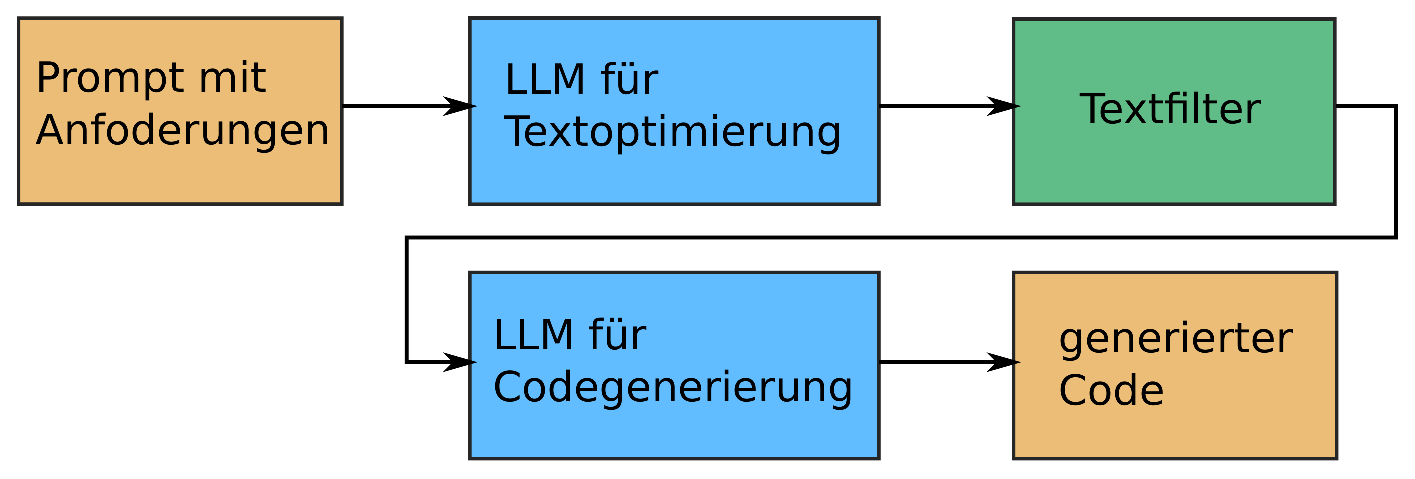
\includegraphics[width=0.8\textwidth]{content/chapter_implementation/images/orchestrierung_llms.eps}
%	\centering
%	\caption{Orchestrierte LLM's für die Codegenerierung}
%	\label{img:orchestration_llms}
%\end{figure}

%\section{Online Modelle}
%Text.

\subsection{Ergebnisse generieren}
Nachdem die Modelle bereitstehen, erfolgt das Generieren der Ergebnisse für jedes einzelne Modell. Mit Prompts, die aus den Proben des HumanEval-XL Benchmark bestehen, werden die Modelle mehrmals hintereinander abgefragt. Die vollständig generierten Antworten der Modelle werden, für eine spätere Auswertung und Nachvollziehbarkeit im \textit{JSONL}-Dateiformat gespeichert. Für jedes Problem erfolgen fünf Abfragen an jedes Modell. Welche Modelle für die Generierung verwendet wurden, ist in Kapitel \ref{subsec:llm_selection} nachzulesen. Alle Modelle wurde von Ollama-Framework bereitgestellt.\vspace{0.2cm}

Für die Optimierung der Prompts wird ebenfalls auf das Ollama-Framework und dessen Modelle zurückgegriffen. Auch hier erfolgt die Kommunikation mit den Modellen über die API.

%-------------------------------------------------------------------------------------------


%\subsection{Auswertung der Modellantworten}
\section{Benchmark Codeevaluation}\label{sec:benchmark_evaluation}
Die Analyse der generierten Antworten muss für jedes Modell individuell angepasst werden, da die erzeugten Codefragmente zwischen den Modellen variieren. Insbesondere unterscheiden sich die Formate, in denen die Codesnippets generiert werden, beispielsweise \texttt{```php} oder \texttt{```php \textbackslash n <?php}. Dementsprechend erfordert die Extraktion des relevanten Codes aus den Modellantworten eine flexible Methode, die an das jeweilige Ausgabeformat angepasst wird. Ein exemplarischer Lösungsansatz zur Extraktion des generierten Codes ist in Listing \ref{lst:evaluation_search_generated_code} dargestellt.\vspace{0.2cm}


Um den generierten Code zu evaluieren, wird dieser und der Test der jeweiligen Probe aus dem Benchmark zusammengeführt. Das Ergebnis ist ein ausführbarer Code, der die geforderte Methode enthält. Mittels Python getestet wird, ob der generierte Code ausführbar ist. Entsteht bei der Ausführung ein Laufzeitfehler erfolgt der Abbruch des Tests. Dieser kann ausgelöst werden durch eine nicht korrekte Syntax, einer Endlosschleife oder wenn die geforderte Methode nicht generiert wurde. All diese Ereignisse führen dazu das die Probe als nicht bestanden gilt. Das Listing \ref{lst:php_interpreter_in_python} zeigt den Ausschnitt im Code zur Ausführung des PHP Interpreters in Python.\vspace{0.2cm}

\begin{lstlisting}[
language=Python,
caption={Codesnippet zur Ausführung des PHP Interpreters},
label=lst:php_interpreter_in_python
]
for answer in answers:
    answer = answer.replace(r"\n", "\n")
    try:
        result = subprocess.run(
            ["php", "-r", f"{test}{sample_result}"],
            capture_output=True,
            text=True,
            check=False,
            timeout=5,
        )
    except subprocess.TimeoutExpired:
        pass

    if result.stderr.strip() == "":
        answer_result_fault = True
\end{lstlisting}

Das unbehandelte Execption-Handling in Zeile 12, dient lediglich dazu, dass die Programmausführung nicht unterbrochen wird und der Test der Probe beendet werden kann. Ein abgelaufener \textit{Timeout} deutet auf eine Endlosschleife hin und somit gilt dieser Test als nicht bestanden. Der hier abgefangene \textit{Timeout} wird in der nachfolgenden \texttt{if} Anweisung mit ausgewertet. Aus den erhaltenen Ergebnissen, berechnet die \texttt{pass@k} Methode eine Vorhersage zur Zuverlässigkeit der jeweiligen vorliegenden Probe, hinsichtlich Codegenerierung. Anschließend wird der Durchschnitt für die Zuverlässigkeit des Modells errechnet.\vspace{0.2cm}

\textbf{Umsetzung der pass@k Metric}\vspace{0.2cm}

Stehen die Ergebnisse aus den Tests fest, werden diese mithilfe der pass@k Methode analysiert. In Python steht, hierfür die Bibliothek \textit{pass\_at\_k} zur Verfügung. Das Listing \ref{lst:custom_pass_at_k} zeigt Umsetzung der Methode nach der Formel \ref{equ:pass_qt_k_complex} aus Kapitel \ref{subsec:pass_at_k}.

\begin{lstlisting}[
	language=Python,
	label=lst:custom_pass_at_k,
	caption={Berechnung der pass@k Metrik in Python}
]
def custom_pass_at_k(n: int, c: int, k: int) -> float:
    """
    :param n (int): numbers of total samples.
    :param c (int): number of currect samples.
    :param k (int): number of consider samples.
    """
    if n - c < k:
        return 1.0
    return 1.0 - np.prod(1.0 - k / np.arange(n - c + 1, n + 1))
\end{lstlisting}

Für die in dieser Arbeit durchgeführten Evaluierungen sind die Werte für $k=1 und k=5$ relevant. Für die Optimierungsaufgaben wird $k=1$ betrachtet. Nachdem jede Probe des HumanEval-XL Benchmark einzeln bewertet wurde, wird eine Zusammenfassung der Bewertung für das gesamte Modell berechnet. Die Berechnung erfolgt nach der Formel \ref{equ:probability_of_success_per_model} aus Kapitel \ref{subsec:pass_at_k}.

% --- More Tests -----------------------------------------------------------------------------------


\section{Codeevaluation mit Frameworks}
\begin{tcolorbox}[
	enhanced,
	colback=red!5!white,
	colframe=red!75!black!50,
	title= Mein roter Faden
	]
	Hier folgen später noch die Evaluierungen der Promptoptimierung.
\end{tcolorbox}

Neben der bekannten Evaluationsmethode mit dem HumanEval Benchmark, wird hier eine weitere Testmethodik überprüft, die mit verschiedenen Validierungstools der jeweiligen Programmiersprache ausgeführt wird. Für die Erstellung der Abfragen wird das Python-Skript verwendet, was schon im Kapitel \ref{sec:benchmark_evaluation} vorgestellt wurde.

\subsection{PHP Codeevaluation}
Der Test wird bei den erweiterten Problemen durchgeführt und beginnt mit den Unit-Tests die mit \textit{PHPUnit} durchgeführt werden. Im Anschluss wird \textit{PHPMetrics} ausgeführt. Hierbei wird geprüft, ob die Codekomplexität und Wartbarkeit überprüft. Die Ausführung der Tests wird mithilfe eines Python-Skripts durchgeführt. Es wird eine PHP Datei erstellt, die mit den Frameworks geprüft wird.

%\subsection{JavaScript Codeevaluation}
%Text.

%\section{Online Modelle}
% Eigenen KI Server \href{https://www.computerweekly.com/de/ratgeber/Einen-KI-Server-mit-Ollama-und-Open-WebUI-einrichte}{Computer Weekly}
% Orchestrierung mit Python \href{https://pypi.org/project/multillm/}{multillm-Projekt}
% LangChain Library \href{https://python.langchain.com/api_reference/ollama/chat_models/langchain_ollama.chat_models.ChatOllama.html}{Example}
% \href{https://pypi.org/project/langchain-ollama/}{Python lib langchain-ollama}
% YouTube \href{https://www.youtube.com/@AICodeKing}{AICodeKing}


\section{Optimierung der Antworten}


\begin{tcolorbox}[
	enhanced,
	colback=red!5!white,
	colframe=red!75!black!50,
	title= Mein roter Faden
	]
	Mögliche Optimierungsstrategien
	\begin{itemize}
		\item mit dem Model Programming (DSPY) Ansatz: Python Bibliothek vorhanden \href{https://pypi.org/project/dspy/}{pypi.org | DSPy}.
	\end{itemize}
\end{tcolorbox}
